\documentclass[./main.tex]{subfiles}

\begin{document}
\section{Simulations} \label{sec:simulations}
In the following section we show the results of applying the two super learners to a simulated dataset. The simulations are carried out using the R programming language and the corresponding source code can be found on the GitHub repository for this project \parencite{github}. The simulated dataset consists of a binary outcome, $Y$, which depends on two covariates $X_1$ and $X_2$. The setup is as follows
\begin{align*}
    X_1 &\sim \operatorname{Unif}(0.5, 15),\\
    X_2 \mid X_1 = x_1 &\sim \mathcal{N}(3.5-0.03x_1, 1),\\
    Y \mid X_1 = x_1, X_2 = x_2 &\sim \operatorname{Ber}(\theta_0(x_1, x_2)),
\end{align*}
for $\theta_0(x_1, x_2) = \expit({-3.5 - 0.3x_1 + 0.85x_2 + 0.35x_1x_2})$ which is the data-generating regression function. It is in fact possible to visualize the regression function explicitly as a 2-dimensional heat map in the covariates. In \Cref{fig:trueplot} we have applied the true regression across the grid of evenly-spaced $ (x_1, x_2) $ covariate pairs in $ (0, 15) \times (0,7) $. The probabilities are colored from $ 0 $ to $ 1 $ in the plot. 
\begin{figure}[H]
    \centering
    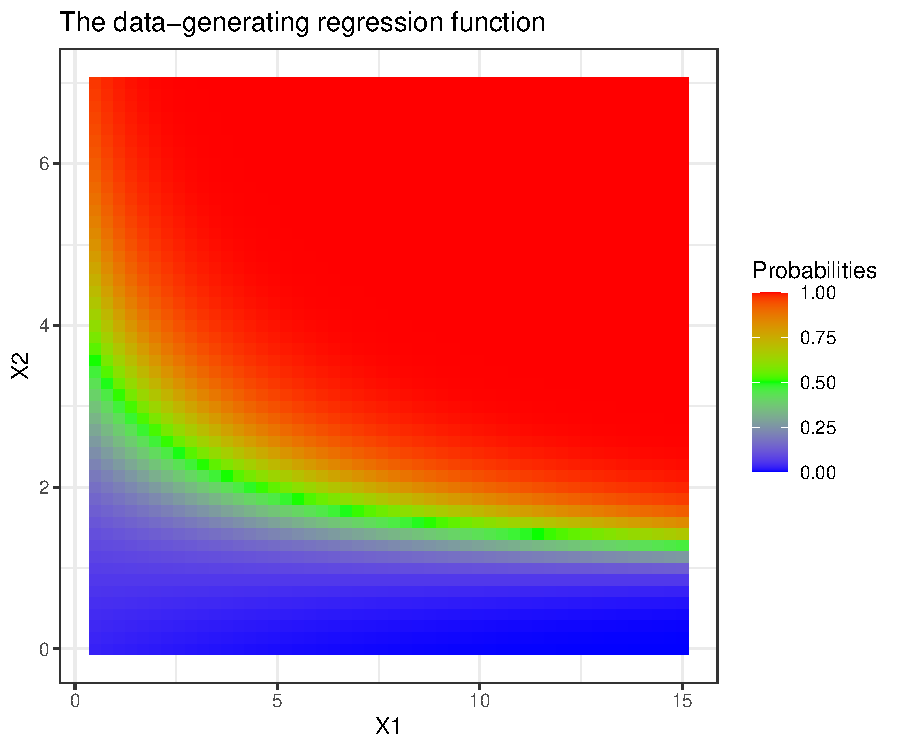
\includegraphics[width=0.8\textwidth]{figures/trueplot.pdf}
    \caption{The data-generating regression plotted as a heat map. The two covariates $ X_1 $ and $ X_2 $ are mapped by the regression function $ \theta_0 $ to a probability as indicated by the colors.}
    \label{fig:trueplot}
\end{figure}
The regression is captured by the logistic regression model with interaction terms. We will use the following library of learning algorithms as an illustrative example:
\begin{enumerate}
    \item Intercept only logistic regression: $E[Y \mid X_1, X_2] = \expit(\beta_0)$
    \item Logistic regression with main effects: $E[Y \mid X_1, X_2] = \expit(\beta_0 + \beta_1 X_1 + \beta_2 X_2)$
    \item XGBoost with hyperparameters: \texttt{max\_depth=3, eta=0.3,\\ n\_rounds=100, objective='binary:logistic', booster='dart', nthread=5}
\end{enumerate}
The intercept only logistic regression is included as a baseline, the predicted probability by the intercept model is simply the sample average over the observed $ Y_i$'s. 

We can visualize the predictions of the learning algorithms in the library in the same way as we have done for the data-generating regression. In \Cref{fig:predictpar} we visualize the predictions of the main effects logistic regression and XGBoost fitted using $1,000 $  observations sampled from the distribution. 
\begin{figure}
    \centering
    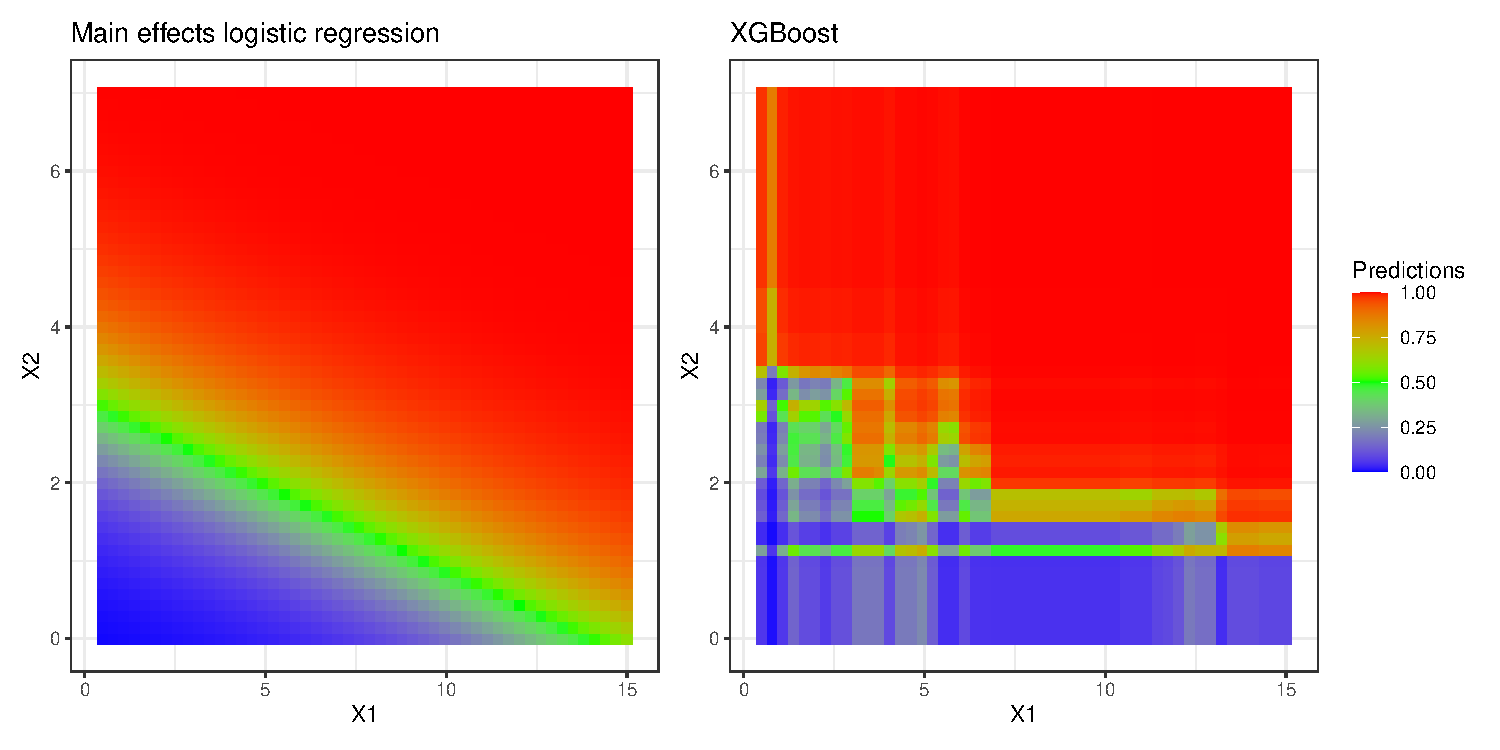
\includegraphics[width=\textwidth]{figures/predictpar.pdf}
    \caption{The predictions of the main effects logistic regression and XGBoost fitted on $ 1,000 $ observations.}
    \label{fig:predictpar}
\end{figure}
The plot for the intercept model is omitted, as its appearance is as one would expect -- the plot is simply an orange square. 

From \Cref{fig:predictpar} we can observe a clear difference in the predicted probabilities between the logistic regression and the tree-based XGBoost. The main effects logistic regression is a parametric model that assumes that the regression function is a smooth transformation of the linear predictor $ X\beta $. XGBoost, in contrast, is made up of many decision trees, which explains the patchwork pattern in its prediction plot. For small samples and as we will see in the simulations, XGBoost has a high risk in comparison to the misspecified main effects logistic regression. However, XGBoost becomes increasingly better at approximating the regression when the number of observations becomes large as seen in \Cref{fig:xgboost10k}. 
\begin{figure}[H]
    \centering
    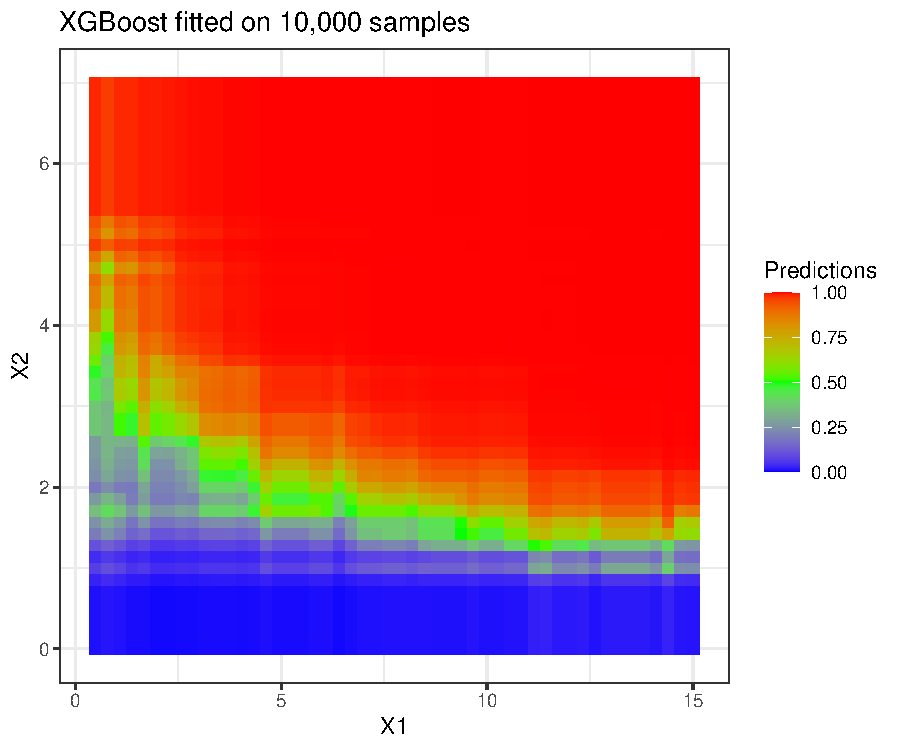
\includegraphics[width=0.8\textwidth]{figures/xgboost10k.pdf}
    \caption{XGBoost becoming better at approximating the regression as the sample size increases. Here the predictions of XGBoost are visualized for a training sample size of $ 10,000 $. They appear to be more stable in comparison to \Cref{fig:predictpar}.}
    \label{fig:xgboost10k}
\end{figure}
\subsection{Discrete super learner} \label{sim_dsl}
By applying the discrete super learning algorithm to the library, we will see that the discrete super learner is able to qualitatively assess and select the best learning algorithm to apply given the amount of data at hand. The discrete super learner uses the main effects logistic regression in the beginning with few training samples, but as the predictions of XGBoost become more stable with more observations, it shifts its preference towards XGBoost. The performance of the discrete super learner will be compared with the learning algorithms in the library on the simulated dataset. We show that:
\begin{enumerate}
    \item As the sample size increases, the discrete super learner achieves the minimum risk 
    \item The variance of the discrete super learner's prediction for a single new observation does not always exhibit a steady descent and depends on the learners in the library
\end{enumerate}

The discrete super learner in our simulations uses 10-fold cross-validation and the internal loss function will be the quadratic loss. While it is possible to do repeated $ K $-fold cross-validation, in our simulations the super learner will only run the cross-validation procedure once given the training data. The following snippet is pseudocode for the discrete super learner algorithm:
\begin{algorithm}[H]
\caption{Discrete super learner}
\begin{algorithmic}[1]
\State \textbf{Input:} $P_n$: dataset, $V$: number of folds, $ \lib $: library of learning algorithms of size $ k $, $ L $: loss function
\State \textbf{Output:} discrete super learner $ \hat{\la}_n(P_n) $
\State $s \gets \text{create random folds}(P_n, V)$ \Comment{Randomly assign observations to folds}
\State $\ell \gets \text{empty array of dimensions } V \times k$ \Comment{Array of risks} 
\For{$s \in \{1, \dots, V\}$}
    \State $P_{n, s}^{1} \gets \{O_i \in P_n \mid s(i) = s\} $
    \State $P_{n, s}^{0} \gets P_n \setminus P_{n,s}^{1} $
    \For{$\la \in \lib$}
    \State $ \la(P_{n,s}^{0}) \gets \text{fit}(\la, P_{n, s}^{0})$
    \State $\ell[s,\la] \gets R(\la(P_{n, s}^{0}), P_{n,s}^{1}) = \frac{V}{n} \sum_{O_i \in P_{n,s}^{1}} L(O_i, \la(P_{n, s}^{0})) $
    \EndFor
\EndFor
\For{$\la \in \lib$}
    \State $ \ell_{\text{avg}}(\la) \gets \frac{1}{V} \sum_{s = 1}^{V} \ell[s,\la] $ 
\EndFor
\State $ \hat{\la}_n \gets \argmin_{\la \in \lib} \ell_{\text{avg}}(\la) $
\State $ \hat{\la}_n(P_n) \gets \text{fit}(\hat{\la}_n, P_n) $  
\State \textbf{return} $ \hat{\la}_n(P_n) $
\end{algorithmic}
\end{algorithm}

\subsubsection{Discrete super learner performance}
The true regression achieves a risk of $ 0.059 $ using the quadratic loss function on a validation set of size $ 10^{6} $. This risk represents the minimum achievable risk for any learning algorithm operating on this dataset. The intercept model -- which is equivalent to predicting an average of the outcomes -- achieves a risk of $ 0.11 $, which serves as a basic benchmark if no effort was made to learn from the data at all. If any learning algorithm performs worse than the benchmark, then it should naturally be discarded from the library.  
\begin{figure}[H]
    \centering
    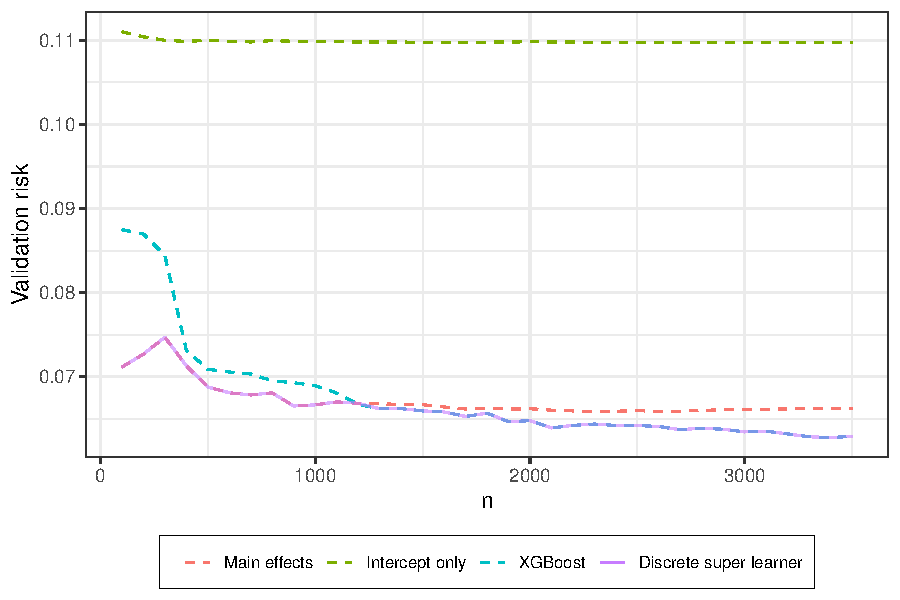
\includegraphics[width=0.9\textwidth]{figures/losses_s22.pdf}
    \caption{The risk of the discrete super learner compared to other algorithms where the number of training samples are $n = 100, 200, \dots , N = 3,500 $. For each $ n $, each learning algorithm is fitted and their validation risks are calculated on a validation set of $ 10^{6} $ observations.} 
    \label{fig:loss_min_of_both}
\end{figure}
\begin{figure}[H]
    \centering
    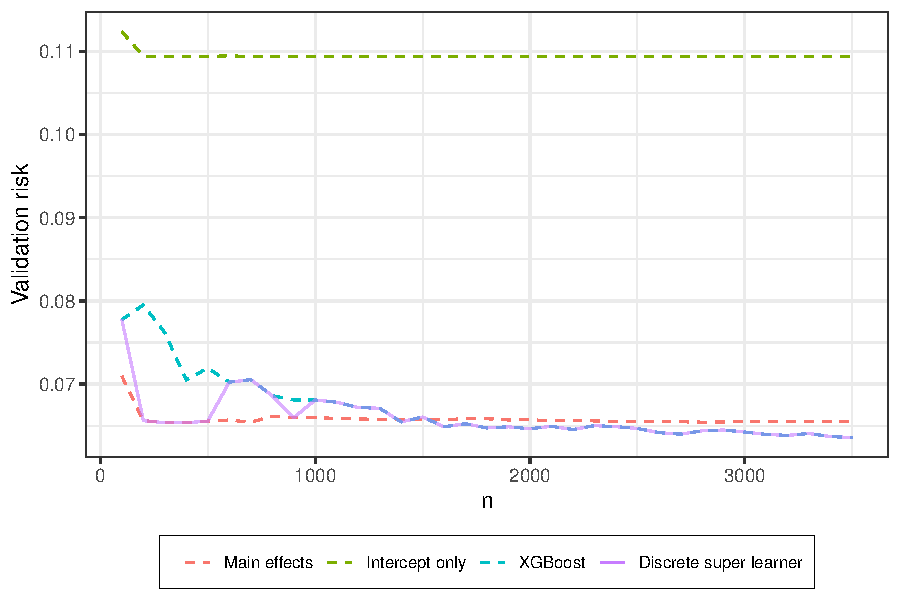
\includegraphics[width=0.9\textwidth]{figures/losses_s23.pdf}
    \caption{Same experiment as illustrated in \Cref{fig:loss_min_of_both} but in another run. The training data is drawn from the data-generating distribution and is therefore subject to seed randomness. The resulting fitted learners will not be the same in the two runs.}
    \label{fig:loss_jumps}
\end{figure}
\pagebreak
\Cref{fig:loss_min_of_both,fig:loss_jumps} demonstrate the performance of the discrete super learner compared to other learners, based on validation risk over the number of training samples. These plots are produced for two runs where the algorithms were fitted on $ n = 100, 200, \dots , N = 3,500 $ observations, as indicated by the horizontal axis. The validation risk is then computed by evaluating each fitted learner on a fixed validation set of $ 10^{6} $ observations sampled from the data-generating distribution.  

The risk for XGBoost is approximately $ 0.062 $ when it is trained on $ 3,500 $ observations. Although this exceeds the optimal risk of $ 0.059 $, it surpasses the main effects model that has a risk of $ 0.066 $. XGBoost evidently outperforms the intercept model, which has a risk of $ 0.11 $. 

The first run provides an excellent demonstration of how the discrete super learner attains the minimum risk. For small training samples, the machine learning method XGBoost has a higher risk than the main effects logistic regression, making the latter a preferable choice for the discrete super learner despite it being misspecified. As a result, the discrete super learner initially achieves the same risk as the logistic regression, but for $ n > 1,200 $ its risk becomes lower. At this point, XGBoost begins to achieve a lower risk than the misspecified logistic regression, leading the discrete super learner to favor XGBoost. 

The second run reveals that the discrete super learner might struggle to determine the learner with the lowest risk when the training sample size is small, causing it to move in a zig-zag pattern between two learners with quite similar risks. However, as the number of training samples increases, the discrete super learner ultimately selects XGBoost.

\begin{figure}[H]
    \centering
    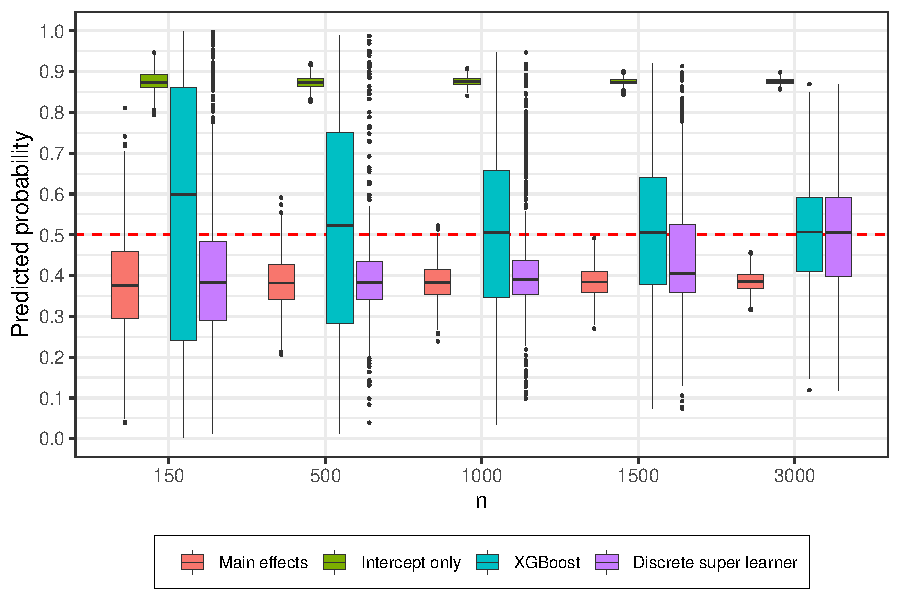
\includegraphics[width=0.9\textwidth]{figures/learner_vars_1000.pdf}
    \caption{Variances of learner predictions for a single observation. Each algorithm is fitted $ K = 1,000 $ times on $n$ samples. Each time they are fitted, they are used to predict on a single fixed observation whose true probability is $ 0.5 $.}
    \label{fig:pred_probs_boxplot}
\end{figure}
\Cref{fig:pred_probs_boxplot} illustrates the variance in the predictions by each learner for a single observation, whose true probability is indicated by the red dashed line at $ p = 0.5 $. Each learner has been trained $ K = 1,000 $ times on $ n = 150, 500, \dots 3,000 $ samples taken from the distribution and is used to predict $ K $ times after each training. The box plots are created from the $ K $ predictions. 

We observe that the machine learning model, XGBoost, has the highest prediction variance across all training sample sizes. Recall that we only had two covariates, here having $ 1,500 $ observations limits the range of predictions of our main effects model to be between $ 0.27 $ and $ 0.46 $, whereas for XGBoost it can vary from below $ 0.1 $ to above $ 0.9 $. While XGBoost is extremely efficient at minimizing loss, its predictions have a high variance unless one has a lot of training data.

Another interesting observation is the bias-variance tradeoff. The parametric learners display low variance, but are highly biased as we see that their predictions are not centered around the true probability at all. On the other hand, XGBoost is much less biased but suffers from a high variance.

The discrete super learner achieves a lower variance than XGBoost for all training sample sizes, which can be attributed to its preference of the low variance main effects logistic regression when the training sample size is small. However, the variance of the discrete super learner increases when $ n \geq 1,000 $ and the box plots become wider. This is due to the discrete super learner's preference of XGBoost as it begins to achieve minimal risk around these number of training samples. 

\begin{figure}[H]
    \centering
    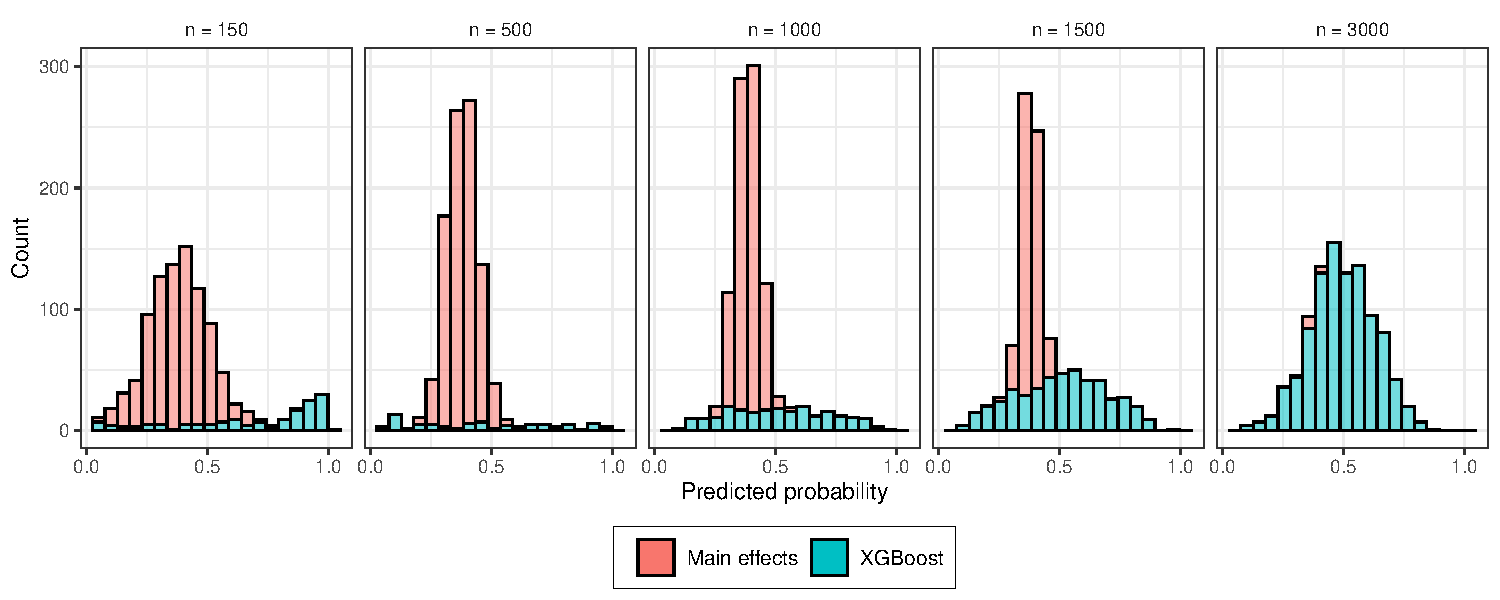
\includegraphics[width=\textwidth]{figures/preds_dsl_shift.pdf}
    \caption{Predictions for a single observation by the discrete super learner varied over the number of training samples $ n $. The predictions are stratified and stacked according to the algorithm that was selected by the discrete super learner.} 
    \label{fig:dsl_shift}
\end{figure}
\Cref{fig:dsl_shift} illustrates how the predictions by the discrete super learner evolves with the number of training samples. The outliers in the discrete super learner box plots from \Cref{fig:pred_probs_boxplot} become evident in this figure. The conclusion here is a reiteration of the points made earlier. In the beginning for $ n = 150 $ to $ n = 500 $ the discrete super learner favors the predictions made by the main effects logistic regression, resulting in a spike in the distribution around $ p = 0.4 $. As the number of training samples increases to $n \geq 1,000$, the discrete super learner assigns more weight to the predictions made by XGBoost, leading to a distribution centered closer to $p = 0.5$. Somewhere between $n = 1,500$ and $n = 3,000$, the discrete super learner becomes confident that XGBoost offers the lowest risk and begins to mirror its predictions.

\subsection{Ensemble super learner} \label{sim_esl}
We will compare the performance of the ensemble super learner with the discrete super learner on the simulated dataset from before. We show that by using the constrained regression meta learning algorithm:
\begin{enumerate}
    \item The ensemble super learner achieves lower risk than the discrete super learner
    \item The ensemble super learner has a lower prediction variance on a single new observations than the discrete super learner
\end{enumerate}

The ensemble super learner will use the same library of algorithms as the discrete super learner, namely the intercept only logistic regression (baseline), the main effects logistic regression and the gradient boosting algorithm XGBoost. The ensemble super learner does internal $ 10 $-fold cross-validation similarly to the discrete super learner, except that the out-of-fold predictions are saved in order to create the level 1 dataset. The following snippet is the pseudocode for the ensemble super learner algorithm:
\begin{algorithm}[H]
\caption{Ensemble super learner}
\begin{algorithmic}[1]
\State \textbf{Input:} $P_n$: dataset, $V$: number of folds, $ \Meta $: meta learning algorithm, $ \lib $: library of learning algorithms of size $ k $
\State \textbf{Output:} ensemble super learner $ \esl(P_n) $
%\State $\ell \gets \text{empty array of dimensions } V \times k$ \Comment{Array of risks} 
\State $\lone_n \gets \text{empty array of dimensions } n \times (k+1)$ \Comment{Level 1 data} 
\State $s \gets \text{create random folds}(P_n, V)$ \Comment{Randomly assign observations to folds}
\For{$s \in \{1, \dots, V\}$}
    \State $P_{n, s}^{1} \gets \{O_i \in P_n \mid s(i) = s\} $
    \State $P_{n, s}^{0} \gets P_n \setminus P_{n,s}^{1} $
    \For{$\la \in \lib$}
        \State $ \la(P_{n,s}^{0}) \gets \text{fit}(\la, P_{n, s}^{0})$
        \For{$ (Y_i, X_i) = O_i \in P_{n,s}^{1} $}
            \State $ \lone_n[i, 1] \gets Y_i $ 
            \State $ \lone_n[i, \la] \gets Z_{i, \la} = \la(P_{n,s}^{0})(X_i) $ \Comment{Save out-of-fold predictions}
        \EndFor
    \EndFor
\EndFor
\State $ \meta \gets \text{fit}(\Meta, \lone_n) $ \Comment{Fit meta learning algorithm on level 1 data}
\For{$\la \in \lib$}
    \State $ \la(P_{n}) \gets \text{fit}(\la, P_{n})$ \Comment{Fit each learning algorithm on all data}
\EndFor
\State $ \esl(P_n) \gets (x \mapsto \meta(\la_1(P_n)(x), \la_2(P_n)(x), \dots , \la_{\ml}(P_n)(x))) $ 
\State \textbf{return} $ \esl(P_n) $
\end{algorithmic}
\end{algorithm}
We visualize the predictions made by the ensemble super learner as we have done in \Cref{fig:predictpar}. \Cref{fig:esl_preds_quad_prog} displays the predictions of the ensemble super learner fitted on $ 1,000 $ and $ 10,000 $ observations using the constrained regression meta algorithm. To do constrained regression we use the R package \textit{lsei} \parencite{lsei}, which is used to solve the quadratic programming problem under constraints.  
\begin{figure}[H]
    \centering
    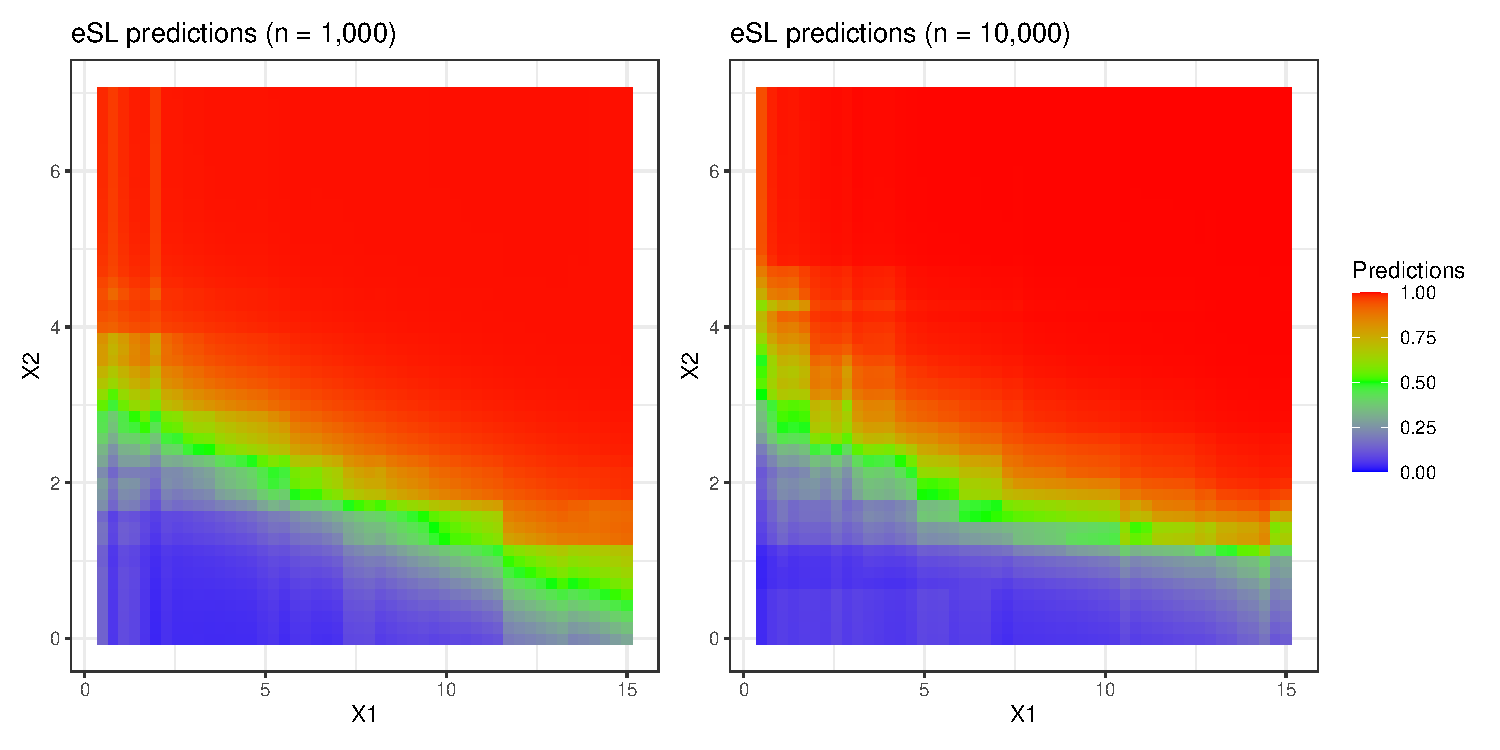
\includegraphics[width=\textwidth]{figures/esl_preds_par.pdf}
    \caption{The predictions by the ensemble super learner using the constrained regression meta learning algorithm fitted on $ 1,000 $ and $ 10,000 $ observations.}
    \label{fig:esl_preds_quad_prog}
\end{figure}
The predictions of the ensemble super learner is a weighted combination of the predictions made by the learners in the library. The contribution from XGBoost is apparent in the patchy pattern that characterizes tree-based algorithms which we touched on before. However, we see that there is a clear gradient in the predictions for $ n = 1,000 $ when transitioning from $ p < 0.5 $ to $ p > 0.5 $, this is likely due to the contribution from the main effects model, which predicts $ p = 0.5 $ along a negatively sloped line through the plot. The weights of the constrained regression can be extracted, in this simulation with $ n = 1,000 $ and $ n = 10,000 $ the fitted weights are: 
\begin{table}[H]
\centering
\begin{tabular}{lcc}
\hline
Learner & $ n = 1,000 $ & $ n = 10,000 $\\
\hline
Intercept & 0.0086 & 0.0001 \\
Main effects & 0.5985 & 0.1366 \\
XGBoost & 0.3929 & 0.8633 \\
\hline
\end{tabular}
\caption{Table of ensemble super learner weights of the different learners}
\end{table}
From the weights we see that the predictions of intercept only logistic regression not important at all for the ensemble super learner. For $ n = 1,000 $ the predictions of the main effects model have the highest weight, which is not surprising in light of our investigations with the discrete super learner, where we saw that the main effects model was more likely to be selected for small samples. Whereas for $ n = 10,000 $ it is weighted a lot less than XGBoost. Note that these weights depend on the data, so they are not necessarily the same when the data is sampled each time. 

\subsubsection{Ensemble super learner performance}
\begin{figure}[H]
    \centering
    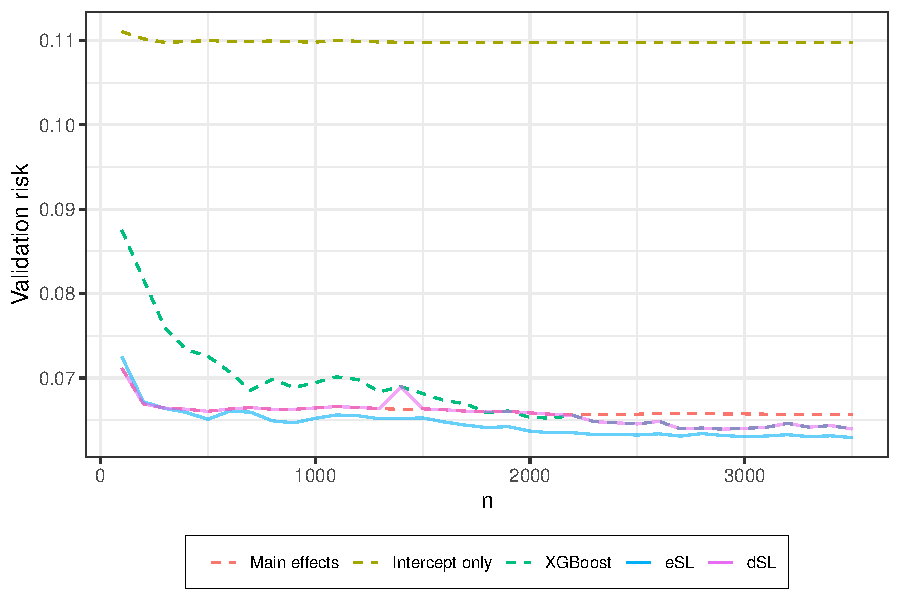
\includegraphics[width=\textwidth]{figures/losses_esl_s22.pdf}
    \caption{The risk of the ensemble super learner compared to other algorithms where the number of training samples are $n = 100, 200, \dots , N = 3,500 $.}
    \label{fig:losses_esl_s22}
\end{figure}
\Cref{fig:losses_esl_s22} demonstrates that the ensemble super learner achieves a lower risk than any of the individual learners, including the discrete super learner. The result agrees with our argument in \Cref{simplex}, where we posited that because the ensemble super learner optimizes across the entire $ \ml $-simplex, its risk is lower compared to the discrete super learner. Nonetheless, it is important to keep in mind that when examining finite samples, the ensemble super learner minimizes risk on the training data, which does not necessarily translate to a lower validation risk. 

As an example, suppose that the library includes the true regression. Limited samples might prohibit the ensemble super learner from assigning full weight to it. The discrete super learner which selects the learning algorithm with the lowest cross-validation risk, might choose the true regression, consequently achieving a lower validation risk than the ensemble super learner.

\begin{figure}[H]
    \centering
    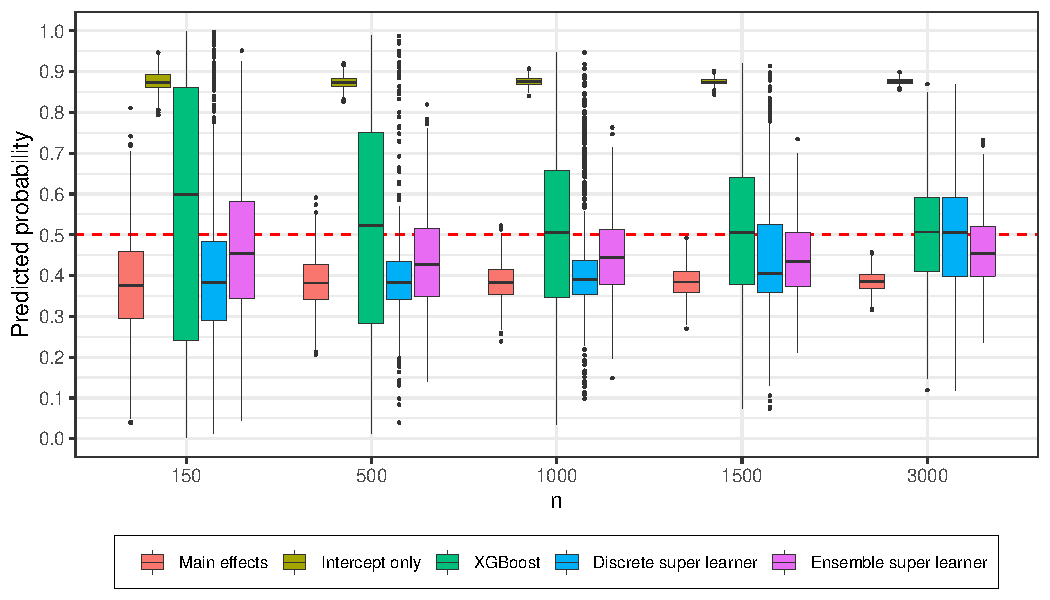
\includegraphics[width=\textwidth]{figures/learner_vars_w_esl_1000.pdf}
    \caption{The variance of the ensemble super learner compared to other learners. Each algorithm is fitted $ K = 1,000 $ times on $n$ samples and used to evaluate $ K $ times on a single observation.}
    \label{fig:learner_vars_w_esl_1000}
\end{figure}
\Cref{fig:learner_vars_w_esl_1000} compares the variances of the ensemble super learner with those of the other learners. Unlike the discrete super learner, which tends to predict many outliers, the predictions of the ensemble super learner have a more centered distribution, as depicted in \Cref{fig:hist_esl_dist}. This behavior is consistent with the fact that the ensemble super learner is a continuous combination of different learners. 

The ensemble super learner appears exhibit a slight bias, albeit less than the parametric learners. Moreover, it maintains lower variance compared to both XGBoost and the discrete super learner, while exhibiting a marginally higher variance than the parametric learners. Thus, it could be argued that the ensemble super learner attempts to balance the bias-variance tradeoff.
\begin{figure}[H]
    \centering
    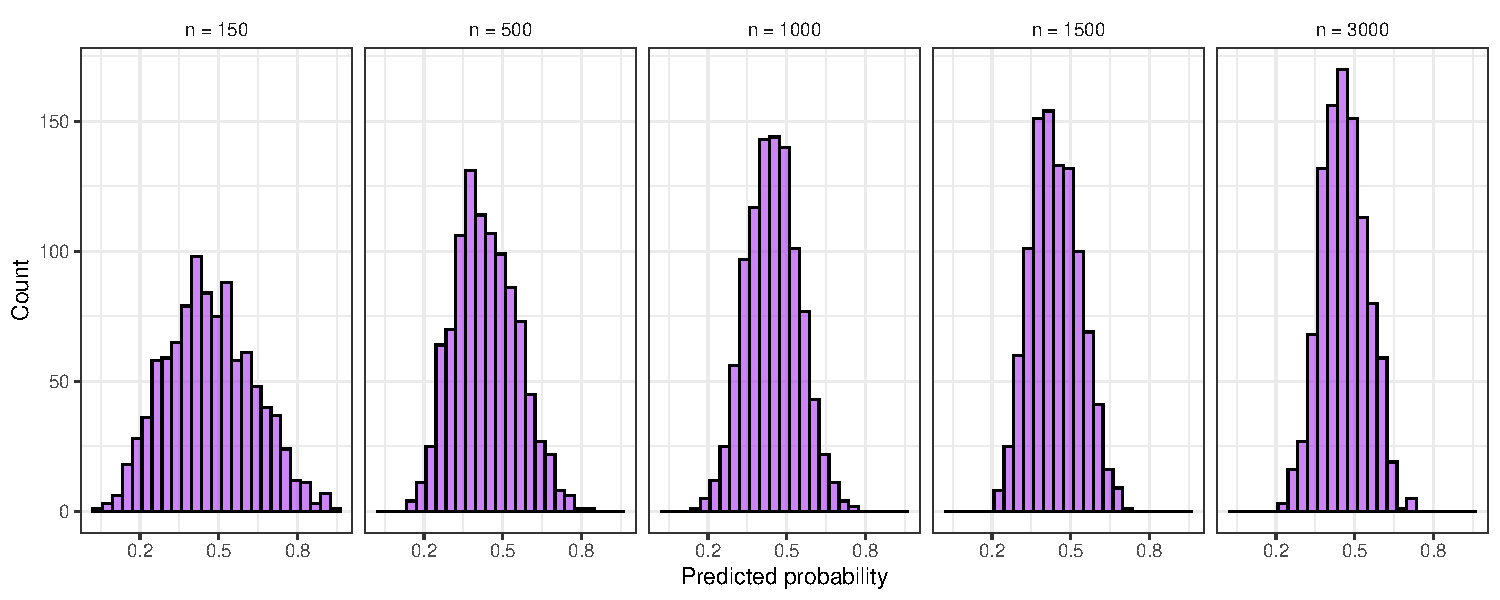
\includegraphics[width=\textwidth]{figures/hist_esl_dist.pdf}
    \caption{Predictions for a single observation by the ensemble super learner varied over the number of training samples. The histograms display the same data as ensemble super learner box plots in \Cref{fig:learner_vars_w_esl_1000}.}
    \label{fig:hist_esl_dist}
\end{figure}
\Cref{fig:hist_esl_dist} shows the predictions of the ensemble super learner for a single observation varied over the number of training samples. We see that the distribution of predictions is much more centered and that the variance seems to also decrease steadily with more samples. 
\begin{figure}[H]
    \centering
    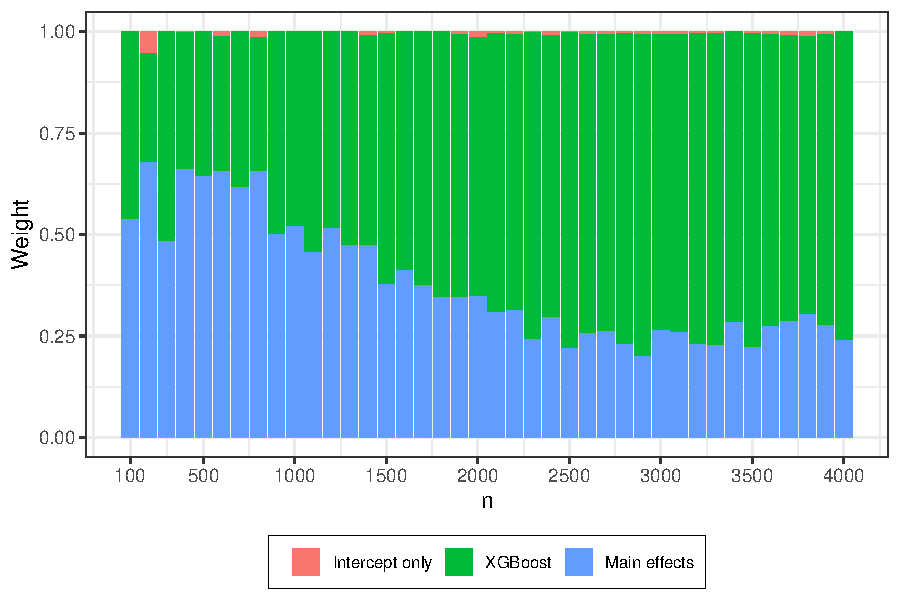
\includegraphics[width=\textwidth]{figures/esl_weights.pdf}
    \caption{Weighting of the 3 different learners selected by the ensemble super learner varied over the number of training samples. The ensemble super learner uses the constrained regression meta algorithm as described in \Cref{simplex}. The weights sum to 1.}
    \label{fig:esl_weights}
\end{figure}
The weighting of the different learners by the ensemble super learner is visualized in \Cref{fig:esl_weights}. We see that the weighting of the intercept only model is very low, and that the main effects model has more weight than XGBoost for small samples. However, this trend reverses as the number of training samples increases. An interesting observation is that XGBoost begins to outweigh the main effects logistic regression when the training size is between $ 1,000 $ and $ 1,500 $, which coincides with when XGBoost begins to achieve a lower risk compared to the main effects model as seen in \Cref{fig:loss_min_of_both,fig:loss_jumps}.

\subsection{Locally weighted ensemble super learner} \label{locally_weighted_ensemble_super_learner}
By using the ensemble super learner with the constrained regression meta learning algorithm we can combine different learners to achieve a lower risk than any of the learners in the library. However, the resulting ensemble is a global combination of the learners, meaning that the weights are the same when predicting on all covariates. In this section I will consider a meta learning algorithm where $ k $-means clustering is used to cluster the covariates into groups and a local weighted combination is fitted for each group.

\subsubsection{Motivation}
By examining the level 1 data obtained from the $ K $-fold cross-validation, it is possible to compare the predictions of each learner against each other as in \Cref{fig:esl_preds_xgboost_vs_main}
\begin{figure}[H]
    \centering
    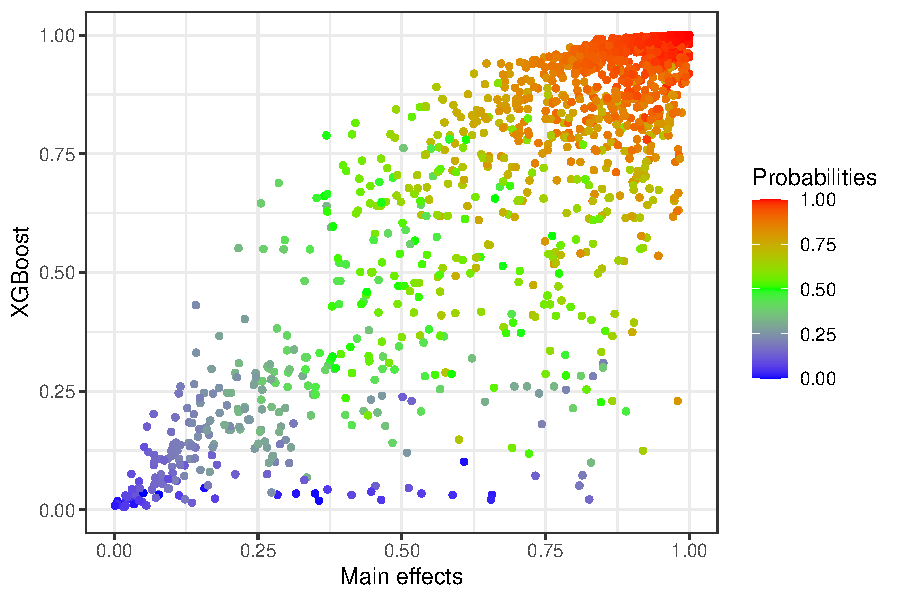
\includegraphics[width=0.68\textwidth]{figures/esl_preds_xgboost_vs_main.pdf}
    \caption{Predictions of XGBoost vs main effects model. The learners' prediction on a single observation represent a point in the unit square, the point is colored by the probability obtained by applying the true regression function on that observation.}
    \label{fig:esl_preds_xgboost_vs_main}
\end{figure}
We notice that the main effects model does not predict the same as the XGBoost. If they had predicted the same, then the predictions would lie on the identity line. There is significant disagreement between the two algorithms, as seen in the lower right corner where the main effects model predicts certain observations to have a probability of over 0.7, while XGBoost assigns these a probability of less than 0.1. An idea is to group the covariates based on the predicted probabilities such that for certain groups certain algorithms are weighed more than others. The naive approach implements $ k $-means clustering to group the covariates into $ k = 4 $ clusters as shown in \Cref{fig:esl_preds_xgboost_vs_main_kmeans} 
\begin{figure}[H]
    \centering
    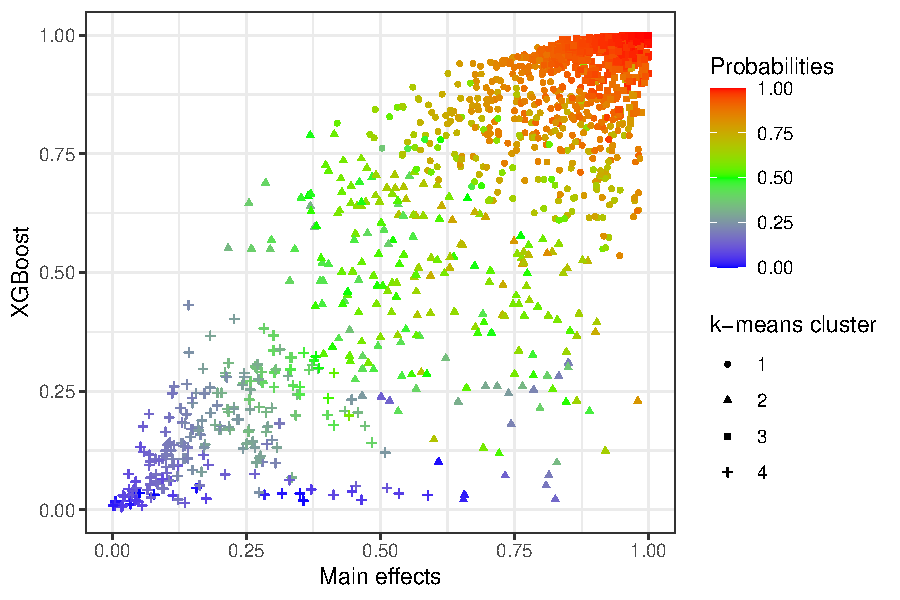
\includegraphics[width=0.68\textwidth]{figures/esl_preds_xgboost_vs_main_kmeans.pdf}
\caption{Same as \Cref{fig:esl_preds_xgboost_vs_main}, except that the observations are clustered into 4 groups using $ k $-means clustering.}
    \label{fig:esl_preds_xgboost_vs_main_kmeans}
\end{figure}
\Cref{fig:esl_preds_xgboost_vs_main,fig:esl_preds_xgboost_vs_main_kmeans} plot the predictions by two learners against each other, but the procedure is valid also when there are more learners, resulting in clustering within a high dimensional space. For each group, a weighted combination of the learners would be found by fitting on the level 1 data of that group. To predict using the ensemble super learner we will apply the learners to the new data and determine which of the clusters the level 1 covariates belong to. Once that has been determined, the predictions will be combined according to the weighted combination in that group. 

\subsubsection{Simulation results}
The locally weighted ensemble super learner examined in this section is implemented with $ k = 4 $ clusters and the same library as in the previous section. The number of clusters was chosen arbitrarily and the results are shown in \Cref{fig:esl_preds_lw}
\begin{figure}[H]
    \centering
    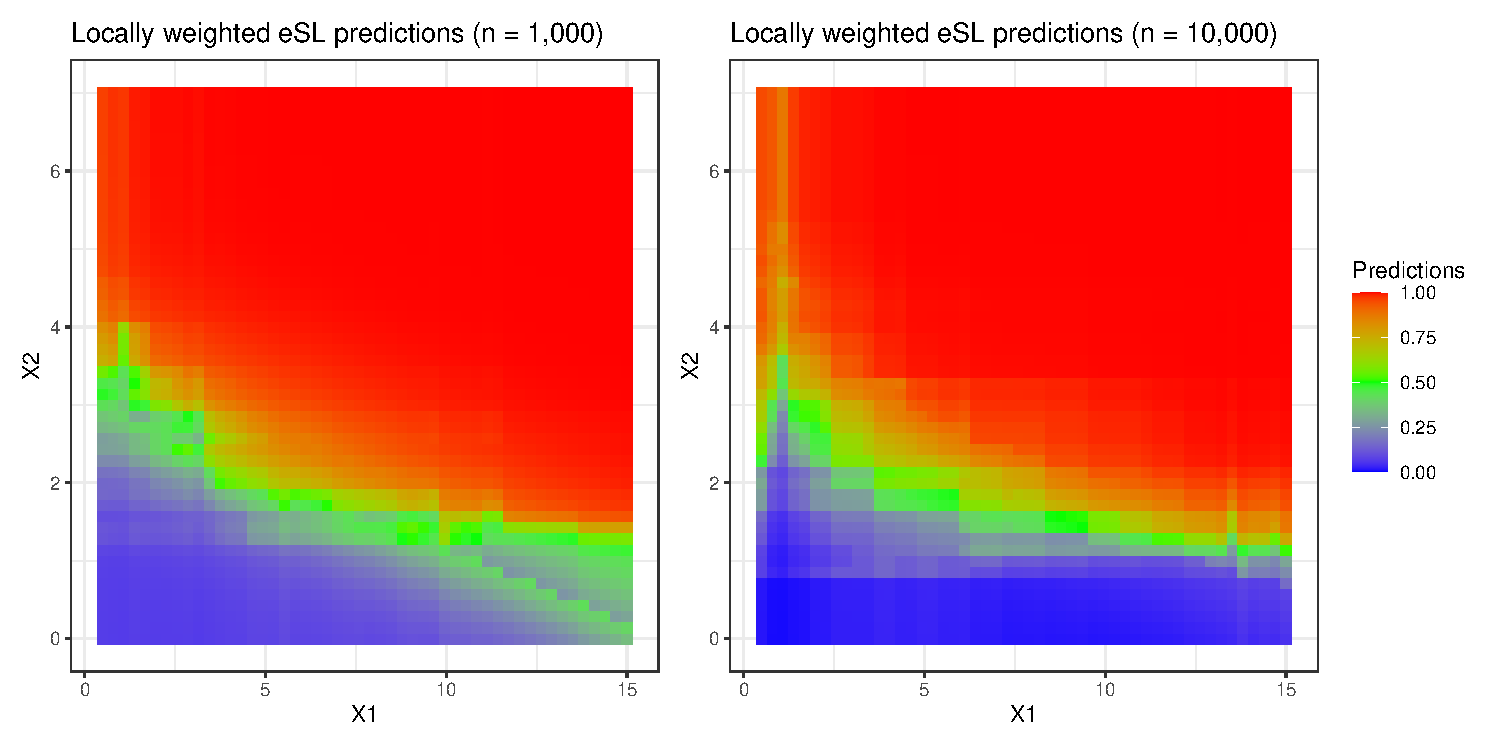
\includegraphics[width=\textwidth]{figures/esl_preds_lw.pdf}
    \caption{Predictions by the locally weighted ensemble super learner fitted on $ 1,000 $ and $ 10,000 $ observations.}
    \label{fig:esl_preds_lw}
\end{figure}
\Cref{fig:esl_preds_lw_stratified} provides a visual representation of the most weighted learner for each point in the covariate grid, where each prediction come from a cluster following a particular weighting scheme. The visualization partitions predictions into two distinct groups: predictions with probabilities above and below $p = 0.5$.

\begin{figure}[H]
    \centering
    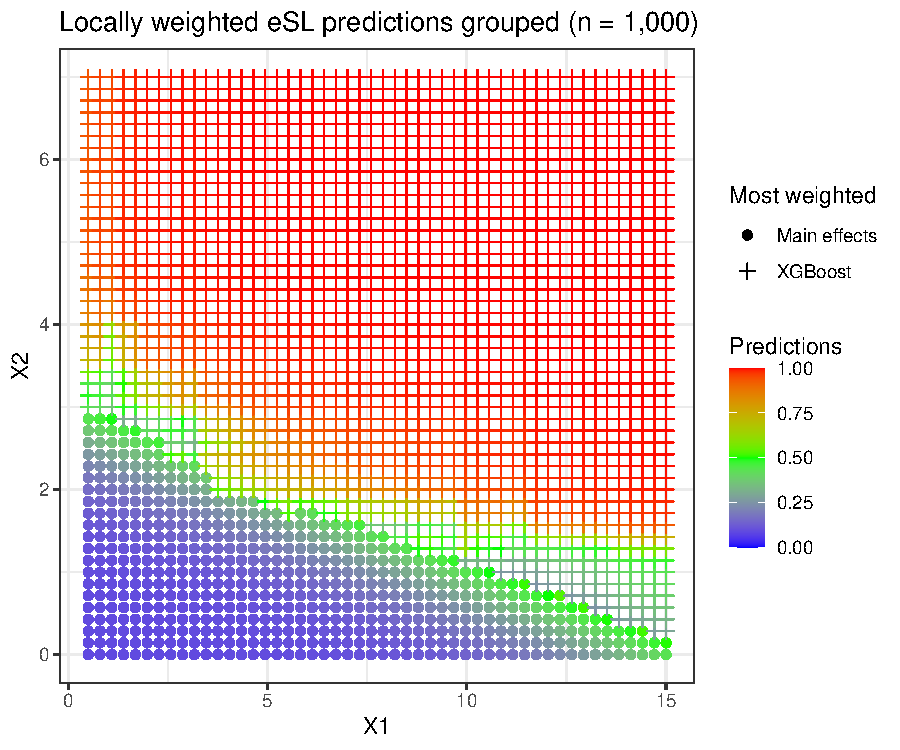
\includegraphics[width=0.8\textwidth]{figures/esl_preds_lw_stratified.pdf}
    \caption{Predictions by the locally weighted ensemble super learner fitted on $ 1,000 $ observations from the left panel in \Cref{fig:esl_preds_lw}, grouped according to the learner with the highest weight. Each colored prediction is a weighted sum of the learner predictions.}
    \label{fig:esl_preds_lw_stratified}
\end{figure}

XGBoost appears to have the highest weight for predictions where the predicted probability is greater than $ 0.5 $, whereas the main effects model is favored when the predictions are below $ 0.5 $. 

The partitioning explains the behavior of the super learner when $ n = 1,000 $ in \Cref{fig:esl_preds_lw}, where it appears that the predictions are smoother for the predicted probabilities less than $ 0.5 $. The explanation is that the super learner weighted the logistic regression the most when $ p < 0.5 $, and since it is a smooth parametric model, the predicted probabilities will assume a gradient. 
\Cref{fig:losses_esl_lw} shows that the locally weighted ensemble super learner has a slightly higher risk than the ensemble super learner, but a lower risk than the discrete super learner. 
\begin{figure}[H]
    \centering
    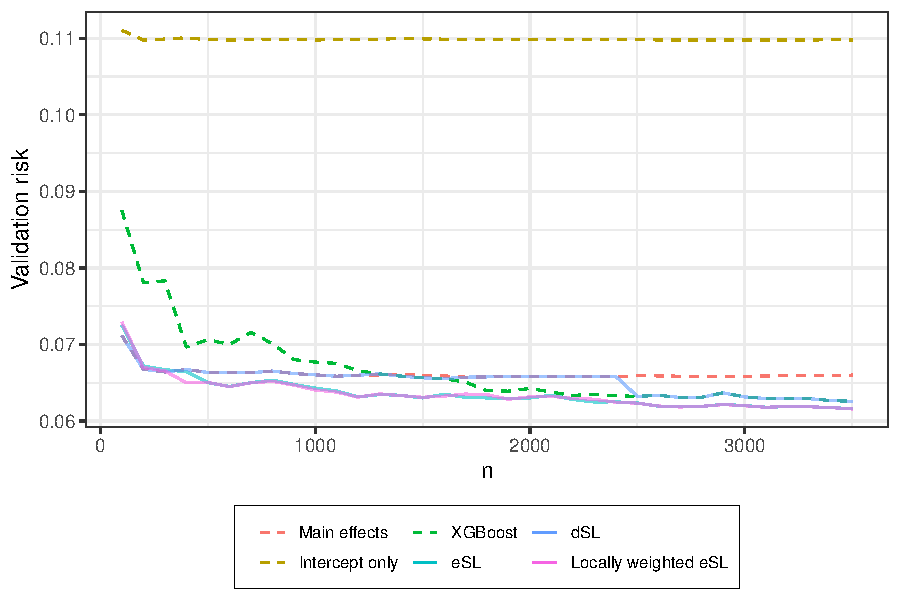
\includegraphics[width=0.9\textwidth]{figures/losses_esl_lw_s22.pdf}
    \caption{The risk of the locally weighted ensemble super learner compared to other algorithms where the number of training samples are $ n = 100, 200, \dots , N = 4,000 $ and $ k = 4 $ local clusters.}
    \label{fig:losses_esl_lw}
\end{figure}
The risk of the locally weighted ensemble super learner can depend on the number of $ k $ clusters that are used to segregate the level 1 data. The connection between the number of clusters and the risk has not been investigated in this thesis. Nevertheless, the risk of a learner does not tell the full picture as we have witnessed with XGBoost, which, despite its design of minimizing loss, displays the highest variance. It might be relevant to consider other metrics that can evaluate the learners on the stability and variance of their predictions. 

\end{document}

